
%%%%%%%%%%%%%%%%%%%%%%%%%%%%%%%%%%%%%%%%%%%%%%%%%%%%%%%%%%%%%%%%%%%%%
%% This is a (brief) model paper using the achemso class
%% The document class accepts keyval options, which should include
%% the target journal and optionally the manuscript type.
%%%%%%%%%%%%%%%%%%%%%%%%%%%%%%%%%%%%%%%%%%%%%%%%%%%%%%%%%%%%%%%%%%%%%
\documentclass[journal=ancham,manuscript=article]{achemso}

%%%%%%%%%%%%%%%%%%%%%%%%%%%%%%%%%%%%%%%%%%%%%%%%%%%%%%%%%%%%%%%%%%%%%
%% Place any additional packages needed here.  Only include packages
%% which are essential, to avoid problems later.
%%%%%%%%%%%%%%%%%%%%%%%%%%%%%%%%%%%%%%%%%%%%%%%%%%%%%%%%%%%%%%%%%%%%%
\usepackage{chemformula} % Formula subscripts using \ch{}
\usepackage{achemso}
\usepackage[T1]{fontenc} % Use modern font encodings
\usepackage{amsmath}
\usepackage{subfigure}
\usepackage{amsfonts}
\usepackage{multirow}

%%%%%%%%%%%%%%%%%%%%%%%%%%%%%%%%%%%%%%%%%%%%%%%%%%%%%%%%%%%%%%%%%%%%%
%% If issues arise when submitting your manuscript, you may want to
%% un-comment the next line.  This provides information on the
%% version of every file you have used.
%%%%%%%%%%%%%%%%%%%%%%%%%%%%%%%%%%%%%%%%%%%%%%%%%%%%%%%%%%%%%%%%%%%%%
%%\listfiles

%%%%%%%%%%%%%%%%%%%%%%%%%%%%%%%%%%%%%%%%%%%%%%%%%%%%%%%%%%%%%%%%%%%%%
%% Place any additional macros here.  Please use \newcommand* where
%% possible, and avoid layout-changing macros (which are not used
%% when typesetting).
%%%%%%%%%%%%%%%%%%%%%%%%%%%%%%%%%%%%%%%%%%%%%%%%%%%%%%%%%%%%%%%%%%%%%
\newcommand*\mycommand[1]{\texttt{\emph{#1}}}

%%%%%%%%%%%%%%%%%%%%%%%%%%%%%%%%%%%%%%%%%%%%%%%%%%%%%%%%%%%%%%%%%%%%%
%% Meta-data block
%% ---------------
%% Each author should be given as a separate \author command.
%%
%% Corresponding authors should have an e-mail given after the author
%% name as an \email command. Phone and fax numbers can be given
%% using \phone and \fax, respectively; this information is optional.
%%
%% The affiliation of authors is given after the authors; each
%% \affiliation command applies to all preceding authors not already
%% assigned an affiliation.
%%
%% The affiliation takes an option argument for the short name.  This
%% will typically be something like "University of Somewhere".
%%
%% The \altaffiliation macro should be used for new address, etc.
%% On the other hand, \alsoaffiliation is used on a per author basis
%% when authors are associated with multiple institutions.
%%%%%%%%%%%%%%%%%%%%%%%%%%%%%%%%%%%%%%%%%%%%%%%%%%%%%%%%%%%%%%%%%%%%%
\author{Valeria Fonseca Diaz}
\email{valeria.fonsecadiaz@kuleuven.be}
\author{Bart De Ketelaere}
\email{bart.deketelaere@kuleuven.be}
\author{Ben Aernouts}
\email{ben.aernouts@gmail.com}
\altaffiliation{Biosystems TC, KU Leuven,
Kleinhoefstraat 4, Geel, Belgium}
\author{Wouter Saeys}
\email{wouter.saeys@kuleuven.be}
\affiliation[KU Leuven]
{KU Leuven, Kasteelpark
Arenberg 30, Leuven, Belgium}
%%%%%%%%%%%%%%%%%%%%%%%%%%%%%%%%%%%%%%%%%%%%%%%%%%%%%%%%%%%%%%%%%%%%%
%% The document title should be given as usual. Some journals require
%% a running title from the author: this should be supplied as an
%% optional argument to \title.
%%%%%%%%%%%%%%%%%%%%%%%%%%%%%%%%%%%%%%%%%%%%%%%%%%%%%%%%%%%%%%%%%%%%%
\title[An \textsf{achemso} demo]
  {Cost-effective model building in multivariate calibration}

%%%%%%%%%%%%%%%%%%%%%%%%%%%%%%%%%%%%%%%%%%%%%%%%%%%%%%%%%%%%%%%%%%%%%
%% Some journals require a list of abbreviations or keywords to be
%% supplied. These should be set up here, and will be printed after
%% the title and author information, if needed.
%%%%%%%%%%%%%%%%%%%%%%%%%%%%%%%%%%%%%%%%%%%%%%%%%%%%%%%%%%%%%%%%%%%%%
\abbreviations{IR,NMR,UV}
\keywords{American Chemical Society, \LaTeX}

%%%%%%%%%%%%%%%%%%%%%%%%%%%%%%%%%%%%%%%%%%%%%%%%%%%%%%%%%%%%%%%%%%%%%
%% The manuscript does not need to include \maketitle, which is
%% executed automatically.
%%%%%%%%%%%%%%%%%%%%%%%%%%%%%%%%%%%%%%%%%%%%%%%%%%%%%%%%%%%%%%%%%%%%%

% -----------------------------------------------------
% -------------------BEGIN DOCUMENT ------------
% -----------------------------------------------------

\begin{document}


% -----------------------------------------------------
% ------------------- abstract  ------------
% -----------------------------------------------------
\begin{abstract}
Multivariate calibration models conceived as virtual sensors that are used to measure chemical compositions in products are built based on spectral data of samples and their corresponding reference chemical values. The cost of these reference analyses is a major of feature of interest to be minimized in industrial applications for the sake of more efficient analytical processes. The present work aims at characterizing the problem of sample selection based on spectral measurements to build calibration models. We mainly focused on evaluating optimal sample sizes, evaluation of different selection methods and we give recommendations on how to assess the suitability of a set of samples to build bilinear calibration models.
\end{abstract}%

% -----------------------------------------------------
% ------------------- introduction  ------------
% -----------------------------------------------------

\section*{Introduction}\label{introduction}

Multivariate calibration models have been the primary analytical tool to indirectly measure the chemical composition of products making processes such as those of quality control more cost-efficient. Many are still the challenges that are present when building and maintaining these models. In the present work, we aim to make an exhaustive evaluation of the problem of unsupervised sample selection to build successful calibration models. This is the type of problem that concerns applications where the product of interest is a collected resource, as it is the case in the agrofood industry (AFI) \cite{Au2020,Diaz-Olivares2020, Saeys2005, Bobelyn2010}.  

The problem of unsupervised sample selection consists in determining what the best methodology or strategy is to select the samples that would be worthy for reference analysis only based on spectral measurements. As it is widely known, spectral measurements are easy and cheap to collect, therefore a vast quantity of units can be submitted to these measurements with low effort. On the contrary, collecting the reference analyses is a task that requires a lot of effort, high costs and possibly high waste. This has been the motivation to pay attention to the optimization of model building costs while gaining model building effectiveness. Historically, the interpretation for this gain has been rephrased as the optimal spread of samples attempting to cover the whole space of variability with a minimum number of samples \cite{Naes1990, Saeys2019,Kennard1969}.

Because of the importance of this problem, up to now there is still research about features such as optimal sample sizes and optimal strategies to select these samples \cite{Au2020, Liu2019}. Through the last decades, many methods have been proposed in light of this problem, some of them becoming widely accepted for their intuitively accurate approach and good performance \cite{Shetty2012a, Nawar2018, He2015}. The two most popular methods in the context of near-infrared (NIR) spectroscopy and multivariate calibration are the Kennard-Stone\cite{Kennard1969} and  Puchwein\cite{Puchwein1988} algorithms. As a strategy, clustering techniques are widely accepted in order to cover the entire variability space\cite{Naes1990}, in particular, when groups of samples exist in batches of collected products\cite{Bobelyn2010}. These popular algorithms have the common feature of relying in distance between the samples. Less popular in NIR applications but highly effective in product design are the optimal design of experiments, which translate the concept of variability from distance between samples to the variance of the coefficients of an assumed model \cite{Goos2011}. Yet, no clear understanding exists about which of all these methods should be used in practice and no exhaustive competition of them has been investigated in NIR applications. The most recent study found attempting to make such a comparison made use of only the two most popular methods mentioned before \cite{Au2020}.

Multivariate calibration is a concept that in principle can involve any type of statistical model. Moreover, both classification and regression models are used in these applications. While the present work focuses on the regression task, the scheme here presented can serve as guidance for classification tasks. Regarding the model architecture, as of now, there is little doubt on the effectiveness of the type of bilinear models that are widely used for NIR applications. Unless the spectral values have a strong nonlinear relationship with chemical reference values, bilinear models such as partial least squares regression (PLSR) or principal component regression (PCR) remain the basic model architectures. Most of the work that can be found addressing the current problem of interest have attempted to answer mainly the question on the minimum required sample size using PLSR models \cite{Naes1990, Au2020, Shetty2012a, Rodionova2008}. The answers that can be found are based on individual applications which leaves a general answer out of the scope. 

In order to have a more general answer on the optimal approach to select a calibration set of samples, it is necessary to think of the application at hand in terms of the statistical models. The general framework of statistical learning theory by Vapnik \cite{Vapnik2019, Vapnik2000} provides specific answers on the sample size needed in light of the model to be used. To deepen into this question for NIR applications, it is necessary to understand PLSR within the framework explained by Vapnik. In a similar way, to understand the required features to take into account for a successful PLSR model, it is necessary to understand which elements of the PLSR architecture can be controlled with unsupervised measurements. These ideas need to be clarified in light of the state-of-the-art strategies for sample selection.

We present here a general and a specific framework of PLSR in order to set a context of analysis to solve the problem of the best strategy for unsupervised sample selection. In the coming sections, we present the frameworks involved together with the research questions that they bring. Afterwards, the experimental work and results are presented along with the discussion and analysis on the aspects that lead to a more successful set of samples to build calibration models.

% -----------------------------------------------------
% ------------------- frameworks  ------------
% -----------------------------------------------------

\section*{Frameworks to understand PLSR}

\subsection*{The general framework}

We aim to put PLSR in the general framework of statistical learning theory. As such, we assume that the response variable is a function consisting in a linear combination and an error variable. With that model architecture, the aim is to minimize a square error \cite{Vapnik2019}. More concretely, let $y \in \mathbb{R}$ be the random variable representing the reference chemical variable of interest and   $\mathbf{x} \in \mathbb{R}^{p}$ the predictor vector of spectral measurements. We assume the relationship $ y = f(\mathbf{x}, \boldsymbol{\beta}) + \epsilon$.  The general regression problem with square error can be established as \cite{Vapnik2000}:

\begin{equation}
    \min E \left[ (y-f(\mathbf{x}, \boldsymbol{\beta}))^2\right]; \quad f(\mathbf{x}, \boldsymbol{\beta}) = \sum_{k=1}^{\infty} \beta_k \phi_{k}(\mathbf{x})
    \label{eq_general_regression_problem}
\end{equation}

where $\{\phi_{i}(\mathbf{x})\}$ constitutes a basis of $L_2$ which can be ordered by some criterion. In terms of the statistical learning theory by Vapnik, $E \left[ (y-f(\mathbf{x}, \boldsymbol{\beta}))^2\right]$ is called the \emph{expected risk} which is in practice replaced by the so-called \emph{empirical risk} in the presence of a set of $n$ observations to estimate function $f$ \cite{Vapnik2000}. In this case, the empirical risk is what has been known for centuries as the sum of square errors. Now, to ensure a small \emph{expected risk}, the \emph{empirical risk} can be minimized only over a limited number of basis functions $\{\phi_{k}(\mathbf{x})\}_{k=1}^d$. Therefore, we are left with a regression problem of the form:

\begin{equation}
    \min \frac{1}{n} \sum_{i=1}^n (y_i-f_d(\mathbf{x}_i, \boldsymbol{\beta}))^2; \quad f_d(\mathbf{x}, \boldsymbol{\beta}) = \sum_{k=1}^{d} \beta_k \phi_{k}(\mathbf{x})
    \label{eq_square_loss_empirical_regression_problem}
\end{equation}

It is therefore in this regard, that the problem as stated in eq. (\ref{eq_square_loss_empirical_regression_problem}) corresponds to the problem that is solved under the PLSR model architecture \cite{Stone1990}, where the basis $\{\phi_{k}(\mathbf{x})\}$ is constructed based on finding the eigenvectors of the covariance between $y$ and $\mathbf{x}$ and are ordered by the amount of covariance. The key element in this framework is the fact that the number of chosen basis functions $d$ represents what Vapnik's theory calls the $VC$ dimension, which is a value that measures the capacity control of a learning machine \cite{Vapnik2019}. The importance of a capacity control value as $d$ for PLSR comes as the reference for determining a suitable sample size when aiming to build a regression machine or as known in the context of chemometrics, a multivariate calibration model. 

In Vapnik's work, it has been stated that we can talk about \emph{small} sample size or a \emph{large} sample size depending on the ratio between the sample size and the $VC$ dimension. Although there is no absolute threshold, it is stated that the sample size is \emph{large} when  $n/d>20$ \cite{Vapnik2000}.


\subsection*{The specific framework}

In the jargon of multivariate calibration, the basis of $L_2$ is what is known as the set of latent variables. Based on a set of $n$ observations stored in the matrices $\mathbf{X}_{n\times p}$ and $Y_{n\times 1}$, the underlying idea of the PLS algorithm is to build latent variables $\{\phi_{k}(\mathbf{x})\}$ such that $\phi_k(\mathbf{x}) = \mathbf{Xv}_{k}$, where $\mathbf{v}_k$ results from maximizing the covariance between $X$ and $Y$ at the $k$-th deflation step. 

For a given value of $d$, the set of resulting latent variables constitute a set of orthonormal variables $\{\phi_{k}(\mathbf{x})\}_{i=1}^d$. However, the set of loading vectors $\{\mathbf{v}_k\}$ is regarded as $\mathbf{S}$-orthogonal, i.e. $\mathbf{v}_k'\mathbf{S}\mathbf{v}_j = 0 \quad (j<k)$, where $\mathbf{S}$ is the covariance matrix of $\mathbf{X}$. The current depiction of the PLSR algorithm clarifies that the estimation of the regression model depends highly on the covariance matrix $\mathbf{S}$ and therefore, when there is availability of a number of spectral measurements $N$, it suggests that it may be possible to select a smaller number of samples $n<N$ for reference analysis such that similar performance is obtained as long as there is equivalence of the matrices $\mathbf{S}$ from the larger sample to the smaller sample, provided that the linear relationship holds true. 

There are several methods and indexes to study the equivalence between two matrices \cite{Tomic2013}. For the sake of bilinear regression models, it becomes manifest to evaluate this equivalence via the spectral value decomposition (SVD) of the matrices. The reason is two-fold. On the one hand, from matrix algebra theory, two matrices are congruent if they have the same eigenvectors
\cite{Horn1985}. On the other hand, the eigenvalues of $\mathbf{S}$ account for the variability that the different dimensions contain and serve as the base to calculate the relative predictive power of the SVD directions (i.e. the PC dimensions) for a regression model \cite{Artemiou2013}. The latter reference is actually referring directly to PCR models, but the present work aims to study the matrix $\mathbf{S}$ for the sake of PLSR models.

% -----------------------------------------------------
% ------------------- research questions  ------------
% -----------------------------------------------------

\section*{Research questions}

When depicting the understanding of PLSR models from a general framework and a specific framework, we see that there are clear elements to take into account at the moment of selecting samples from a large set of available spectral measurements to build calibration models. On the one hand, the $VC$ dimension comes as a reference value for the sample size. On the other hand, if $N$ spectral measurements are available, we may be able to determine the quality of a set a subset of these samples of size $n<N$ based on the equivalence of the covariance matrices $\mathbf{S}$ for $N$ and $n$ samples. With this in mind, we aim to study the following aspects:

\begin{itemize}
    \item Can we find particular thresholds regarding the optimal sample size for satisfactory PLSR models in chemometrics based on the ratio $n/d$?

    \item Is there any relationship between eigenvectors and eigenvalues of $\mathbf{S}_N$ and $\mathbf{S}_n$ as a function of the sample size?
    
    \item What are the most suitable sample selection conditions in light of satisfactory PLSR models?
\end{itemize}

% -----------------------------------------------------
% ------------------- experimental  ------------
% -----------------------------------------------------

\section*{Experimental}\label{experimental}

\subsection*{Case studies}\label{data}

We selected two AFI real case studies to demonstrate the aspects previously discussed about unsupervised sample selection. The first one corresponds to the inspection of milk composition where data of 2 periods of time were available both for spectral signals and reference analysis \cite{Diaz-Olivares2020}. During the first period 316 samples were collected followed by 79 new samples collected in the second period. The time frame between the periods was two weeks. The spectral measurements correspond to transmittance mode gathered in the range 900 nm - 1700 nm with a resolution of 3 nm. In this case the chemical variable of interest was lactose. 
The second case corresponds to pig manure samples collected in 2015 where 2 sets were available for the inspection of the manure composition \cite{Saeys2005}. One set of 420 samples was measured under the same conditions for calibration and a separate set of 164 samples was measured for validation. The chemical constituent chosen for inspection through calibration was Dry Matter. The spectral measurements correspond to reflectance model in the range 426 nm - 1686 nm with a resolution of 9 nm.
For the purpose of analyzing the sample selection problem, we refer to the first sets in both cases as selection set, the samples chosen by the different methods constitute the calibration set and the samples on the second sets represent the test set. The descriptive statistics of the sample sets are shown in Table \ref{tab_descriptive_statistics}.

\textbf{Preprocessing:} For the purpose of studying unsupervised sample selection for satisfactory calibration models, only mean centering preprocessing was used in all cases. Based on initial experiments, it was seen that assuming certain preprocessing filters for the spectral measurements prior to any knowledge of the $y$ values might be harmful for the resulting model. 

\begin{table*}[t]
\centering
\begin{tabular}{|c|c|c|c|c|} 
\hline
Case study	& set & size & mean($y$) & std($y$)  	\\
\hline
\multirow{2}{10em}{Milk ($y$: lactose (\%))} & selection & 316 & 4.7371 & 0.1547\\
& test & 79 & 4.7044 & 0.1554\\
\hline
\multirow{2}{10em}{Manure ($y$: DM (-))} & selection & 420 & 66.0224 & 34.7173\\
& test & 164 & 64.2887 & 38.5147 \\
\hline 


\end{tabular}
\caption{Descriptive statistics}
\label{tab_descriptive_statistics}
\end{table*}

\subsection*{Methodology}\label{methodology}

\subsubsection*{Exhaustive evaluation for unsupervised sample selection}

We set up an exhaustive evaluation consisting in combining three main factors involved into the problem of interest: Method, input dimensionality and sample size. We aimed to evaluate the impact of each of these factors on model performance by selecting subsets of samples for each possible combination of these factors. We explain here the definition of each factor and their possible values are listed in Table \ref{tab_samplesel_settings_exhaustive_search}.

\textbf{Selection methods}

There are multiple methods in the state of the art for sample selection based on the available matrix $\mathbf{X}$. After revising the literature on chemometrics and calibration models, the methods selected for the present work were: Kennard Stone (KS) \cite{Kennard1969}, Duplex (DUP) \cite{Snee1977}, Puchwein (PUCH)\cite{Puchwein1988}, complete linkage hierarchical clustering (CL) \cite{Naes1990} and D-optimal designs based on the Federov algorithm (D-OPT) \cite{Goos2011}. In addition, we included random selection (RAND). 

\textbf{Input dimensionality}

The available spectral measurements stored in matrix $\mathbf{X}_{N\times p}$ correspond to an input dimensionality of $p$. However, due to the rank deficit of $\mathbf{X}$, it is also possible to reduce the input dimensionality for sample selection via principal component analysis (PCA) scores, therefore defining an input matrix $\mathbf{T}_{N\times a}$ of $a$ PC scores, which sets a range for the input dimensionality $a$. The value of $a$ should not be confused with the $VC$ dimension for the PLSR model $d$. Based on the evaluation of the current cases and results seen in the literature of chemometrics, the range of $a$ was set from 1 to 25 in addition to $a=p$. 

\textbf{Sample size}

Based on the maximum number of principal components ($a=25$), the minimum sample size was set to 30 samples. The sample size range was considered in steps of 10 from 30 to the maximum number of samples available in the selection set for each case study. 

\textbf{Constraints}

For the distance-based selection methods (KS,DUP,PUCH,CL), a mahalanobis distance was used for $a=1,...,25$ and a euclidean distance measure was used for $a=p$. This is decided because the inverse of the covariance matrix $\mathbf{S}$ if $a=p$ to be used in the mahalanobis distance becomes highly unstable due to its rank deficiency. For the same reason, the selection based on D-OPT can be made only for $a=1,...,25$. 

\begin{table*}[t]
\centering
\begin{tabular}{|c|c|c|} 
\hline
Selection method	& Input dimensionality	& Sample size	\\
\hline

KS & 1 PC   & 30  \\
DUP &  . & 40\\
PUCH &  . & . \\
CL & . & . \\
D-OPT & 25 PC's & .\\
RS & $p$ & $N$\\
\hline


\end{tabular}
\caption{Sample selection settings}
\label{tab_samplesel_settings_exhaustive_search}
\end{table*}

\subsubsection*{Analysis of covariance matrix $\mathbf{S}$}

We evaluated the equivalence or congruence between the covariance matrix based on the full available sample of size $N$ ($\mathbf{S}_N$) and a covariance matrix based on a subset of size $n$ ($\mathbf{S}_n$) through the correspondence of their eigenvectors and the eigenvalues. The spectral value decomposition of $\mathbf{S}_N = \mathbf{V_N \Delta_N V'_N}$ and $\mathbf{S}_n = \mathbf{V_n \Delta_n V'_n}$ was calculated. The eigenvalues were compared by calculating the ratio  $\Delta_n/\Delta_N$ and the eigenvectors were compared by computing the absolute value of the determinant for the matrix $V'_nV_N$ setting a value for the rank. As the set of eigenvectors constitutes also an orthonormal basis, this determinant takes an absolute value between 0 and 1. In addition, Pearson correlations between $y$ and the SVD dimensions (i.e. PC scores) were calculated to show the impact of dimensions of small variability.

\subsubsection*{Multivariate calibration models}

The PLSR models were trained using the SIMPLS algorithm \cite{DeJong1993}. For each selection setting as explained in Table \ref{tab_samplesel_settings_exhaustive_search}, a PLSR model was calibrated with the selected samples and applied on the separated test set for each case study. The performance of the model corresponded to the root mean squared error (RMSE)  on 10-fold crossvalidation and the test set in a range from 1 to 30 latent variables. 

\subsection*{Computational tools}

The complete analysis was programmed and run in Python 3.7. The selection methods, excluding D-OPT, were programmed in house as well as the SIMPLS algorithm. The D-OPT method was used in a connection from R to Python, using the function \texttt{optfederov} from the R-package \emph{AlgDesign}\cite{Wheeler2019}. The exhaustive sample selection and subsequent PLSR calibrations was embedded into a loop which was highly optimized using \texttt{numba} for Python \cite{Lam2015}. It was possible to fit more than 5000 PLSR models including crossvalidation results in 10 minutes in an 64-bit Inter Core i7 vPro 8th generation with 16 GB of RAM. 


% -----------------------------------------------------
% ------------------- results  ------------
% -----------------------------------------------------

\section*{Results}\label{results}

\subsection*{General framework}\label{results:genframework}

\emph{Can  we  find  particular  thresholds  regarding the optimal sample size for satisfactory PLSR models in chemometrics based on the ratio $n/d?$}

We aimed to answer this question by gathering the results in terms of performance from all the models calibrated in the exhaustive evaluation. In total, for the Milk case there were 5360 models and for the Manure case there were 7210 models. In order to show the effect of the the ratio $n/d$, an \emph{optimal} complexity $d$ needed to be established. Such an optimal complexity was chosen based on the performance in crossvalidation (RMSECV) and prediction error (RMSEP) when using the total number of samples available in the selection set. Figure \ref{fig_d01_milk_general_framework} (a) shows the RMSE curves for crossvalidation and test where it can be seen that for lactose the optimal complexity happens to be between 16 and 18 \cite{Diaz-Olivares2020}. Therefore, to analyze the ratio $n/d$ using the lactose prediction, $d$ was fixed as 16,17 and 18 latent variables. In the case of Manure, the same choices were made based on the RMSE curves shown in Figure \ref{fig_d02_manure_general_framework} (a). Taking the separation between RMSECV and RMSEP and the increasing point for each curve, the optimal complexity for DM was set as $d = 11,12,13 \text{ and } 14$ using only mean-centering preprocessing \cite{Saeys2005}. 

Figures \ref{fig_d01_milk_general_framework}(b) and \ref{fig_d02_manure_general_framework}(b) show the RMSEP values as a function of the ratio $n/d$ for the chosen optimal complexities in each case study. To answer the current question, it was observed that when gathering all the possible sample selection possibilities, there is a clear stabilization of the prediction error as a function of the ratio of interest. Before a ratio of 10, there is clear uncertainty in the prediction performance of the models, where therefore the sample size was small compared to the optimal complexity of the calibration model. However, in the prediction of lactose, a stabilization threshold could be obtained as $n/d>12$ obtaining similar performance as reported in previous works\cite{Diaz-Olivares2020, Aernouts2011}. Because of the available number of samples (316), for the chosen optimal complexity, the maximum ratio could not surpass 20. Interestingly, a similar result was observed in the prediction of DM. A jump was observed after a ratio of 12 and then a final stabilization point was detected as $n/d>16$ reaching similar performance as obtained in the reference work\cite{Saeys2005}. In both of the cases, the highest uncertainty for the performance of the calibration model was obtained in $n/d<10$. For these specific cases, this insight suggests that if the model complexity for lactose would not be less than 16 latent variables, the minimum sample size is $16*10=160$. For the case of DM, the minimum sample size should then not be less than $11*10=110$. 

\begin{figure}[b]
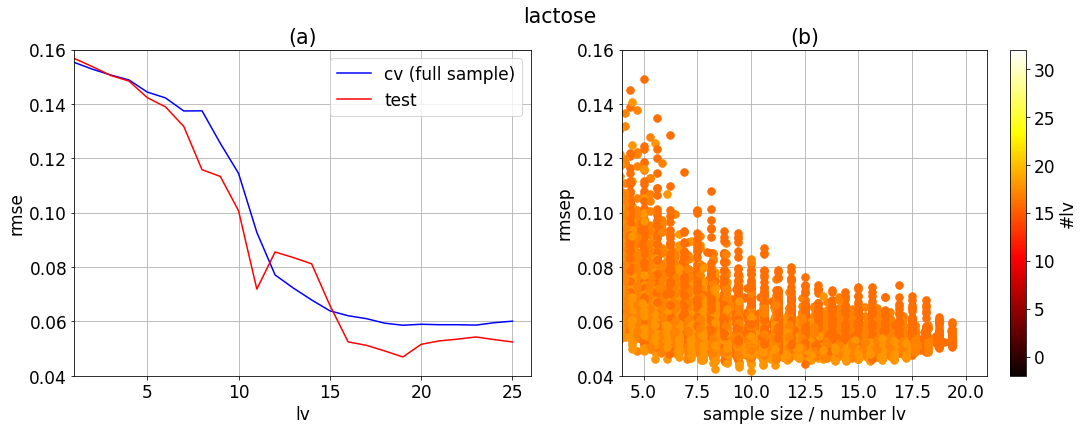
\includegraphics[width=0.8\textwidth]{manuscript/figures/d01_milk_general_framework.png}
\centering
\caption{(a) RMSECV based on the complete selection set and RMSEP for Milk data set. (b) RMSEP values as function of the ratio $n/d$ for 16, 17 and 18 latent variables as indicated in colorbar.}
\label{fig_d01_milk_general_framework}
\end{figure}

\begin{figure}[b]
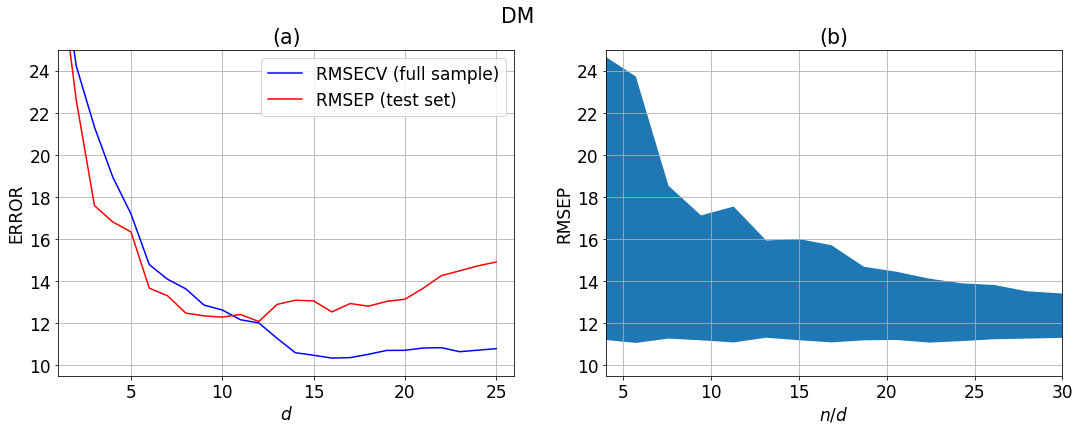
\includegraphics[width=0.8\textwidth]{manuscript/figures/d02_manure_general_framework.png}
\centering
\caption{(a) RMSECV based on the complete selection set and RMSEP for Manure data set. (b) RMSEP values as function of the ratio $n/d$ for 11 to 14 latent variables as indicated in colorbar}
\label{fig_d02_manure_general_framework}
\end{figure}

\subsection*{Specific framework}\label{results:specframework}

\emph{Is there any relationship between eigenvectors and eigenvalues of $\mathbf{S}_N$ and $\mathbf{S}_n$ as a function of the sample size?}

As stated in the introduction for the specific framework, the mathematical element that can be controlled to calibrate PLSR models is $\mathbf{S}$, the covariance matrix of $\mathbf{X}$. The analysis of equivalence or congruence between $\mathbf{S}_N$ and $\mathbf{S}_n$ was done by comparing the eigenvectors and eigenvalues of the matrices. Figure \ref{fig_specific_framework_detereigevect} shows the comparison of the eigenvectors of $\mathbf{S}_N$ and $\mathbf{S}_n$ for both of the case studies when the sample selection was made with $a=15,20,\text{and} 25$with each method. These values of $a$ corresponded to rank values going beyond the number of dimensions that accumulate more than 99.99\% of variance in both case studies.

Across the different methods, the determinant to be evaluated was higher than 0.8 for sample sizes less than 100 in both case studies when setting the rank $a=15 \text{and} 20$. Likewise, across the methods, there was an evident difference in the behavior of the determinant for $a=25$. In both case studies, CL and D-OPT selection showed a jump in the determinant around the same sample sizes. This was not the same behavior for the other selection methods. As expected, due to the nature of selection with DUP, the determinant presents a declination after crossing 50\% of the samples for selection. However, this decline was obtained for $a=20, 25$ and not for $a=15$ making evident the effect of the input dimensionality.   

The second part in analyzing the equivalence of covariance matrices corresponded to the comparison of the eigenvalues. Figure \ref{fig_d01_milk_specific_framework_eigenvalsratio} shows the comparison of the eigenvalues at each dimension for the Milk case across selection methods and selecting with $a=25$. The curves are colored by the sample size. In this comparison, the same effect of the Duplex algorithm is detected as the ratio of the several eigenvalues goes under 1 which translates into an underestimation of the variability at that particular direction compared to the variability based on total sample.  The selection under KS, D-OPT and PUCH show that in general there is no underestimation of variability as the eigenvalues ratio stays above 1 except one dimension with the smallest sample size. For all the methods except RAND, the selection with small sample sizes clearly shows that there is no uniform spanning of the variability as some dimensions result in eigenvalues ratios are twice as large as others. Most interestingly, this discrepancy happens at the same specific directions of the SVD across the selection methods.

As CL is a more robust method compared to the other methods in terms of control over possible outliers, the eigenvalues ratio is overall more stable and closer to 1 in comparison with the other methods. In fact, for some directions when keeping a small sample size, the ratio went quite under 1. D-OPT showed more linearity for the ratio as a function of the sample size compared to the other methods and being generally also the highest ratio values. This result is expected as the nature of selection by D-OPT is exactly the expansion of variability of the SVD directions.  

The behavior of the different methods described for the Milk case were observed also in the analysis of the Manure case as shown in Figure \ref{fig_d02_manure_specific_framework_eigenvalsratio}. It was seen that indeed D-OPT managed to keep the ratio linearly higher as a function of the sample size than the other methods did. This result was particularly clear for the later SVD dimensions. The expansion of variability for those late directions was kept lower with CL selection than with other methods except RAND.  

To complement this analysis, Pearson correlations were calculated between the SVD dimensions and the $y$ variables in both case studies. Table \ref{tab_correlations} shows the correlations for different dimensions. In the case of Milk, PC's 18 and 21 showed higher correlations with lactose than even PC's 1 and 2. In the case of Manure, DM had a higher correlation with PC 5 than PC 1. For applications such as the Milk case study it was observed that there is a high correlation with late PC's which are mostly underestimated compared to first PC's, based on the resulting eigenvalues ratio results for the different methods. Finally, the random selection proved to be in no real relation with the sample size, presenting highly oscillating results for small sample sizes and getting stable around 1 as the sample size is close to the total sample. 


\begin{table*}[t]
\centering
\begin{tabular}{|cc|cc|} 
\hline
\multicolumn{2}{|c|}{Milk (lactose)} & \multicolumn{2}{|c|}{Manure (DM)}\\
\hline
pc	& correlation	&  pc & correlation	\\
\hline
  1 & -0.1337 & 1 & -0.3132 \\
  2 & -0.1839 & 2 & -0.6231 \\
  3 & -0.0239 & 3 & -0.1587 \\
  4 &  0.2380 & 4 &  0.2220 \\
  5 &  0.0496 & 5 &  0.4036 \\
 16 &  0.0060 & 6 &  0.0299 \\
 17 &  0.0266 & 7 & -0.3102 \\
 18 &  0.4208 & 8 & 0.0521 \\
 19 &  0.1202 & 9 & 0.1543 \\
 20 &  0.0759 & 10& 0.0259 \\
 21 &  0.3819 &  & \\
 \hline
\end{tabular}
\caption{Pearson correlations between PC's and chemical component based on the selection set}
\label{tab_correlations}
\end{table*}


\begin{figure*}[t]
    \centering
    \subfigure[Milk]{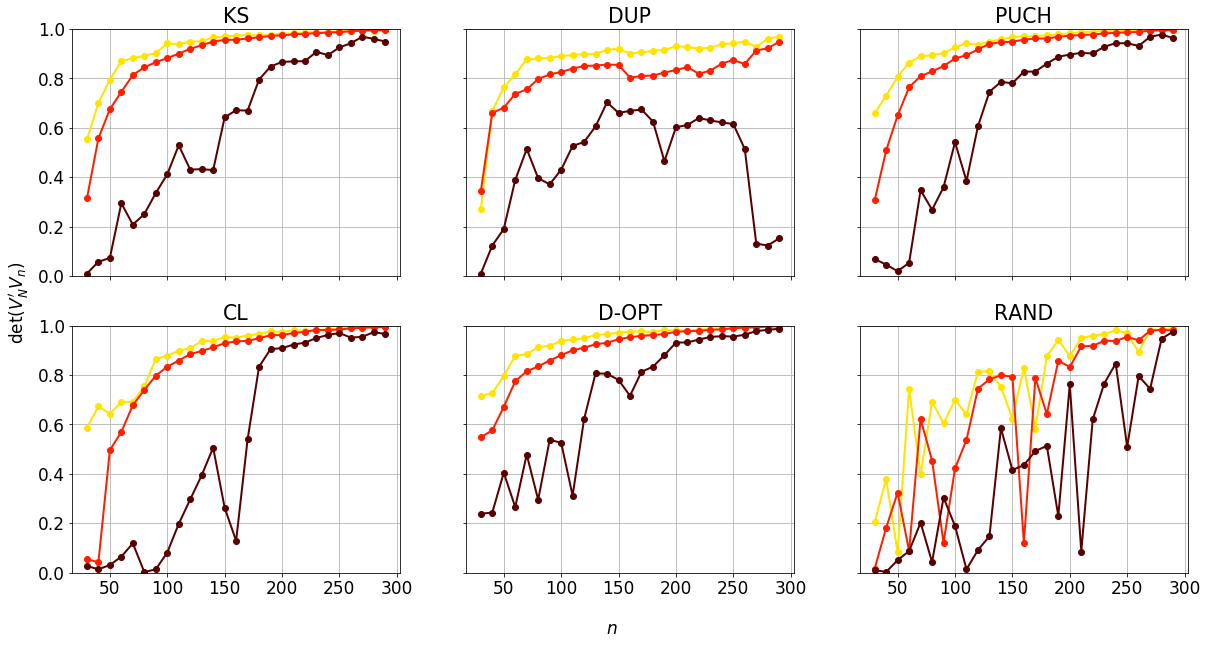
\includegraphics[width=0.6\textwidth]{manuscript/figures/d01_milk_specific_framework_detereigevect.png}} 
    \subfigure[Manure]{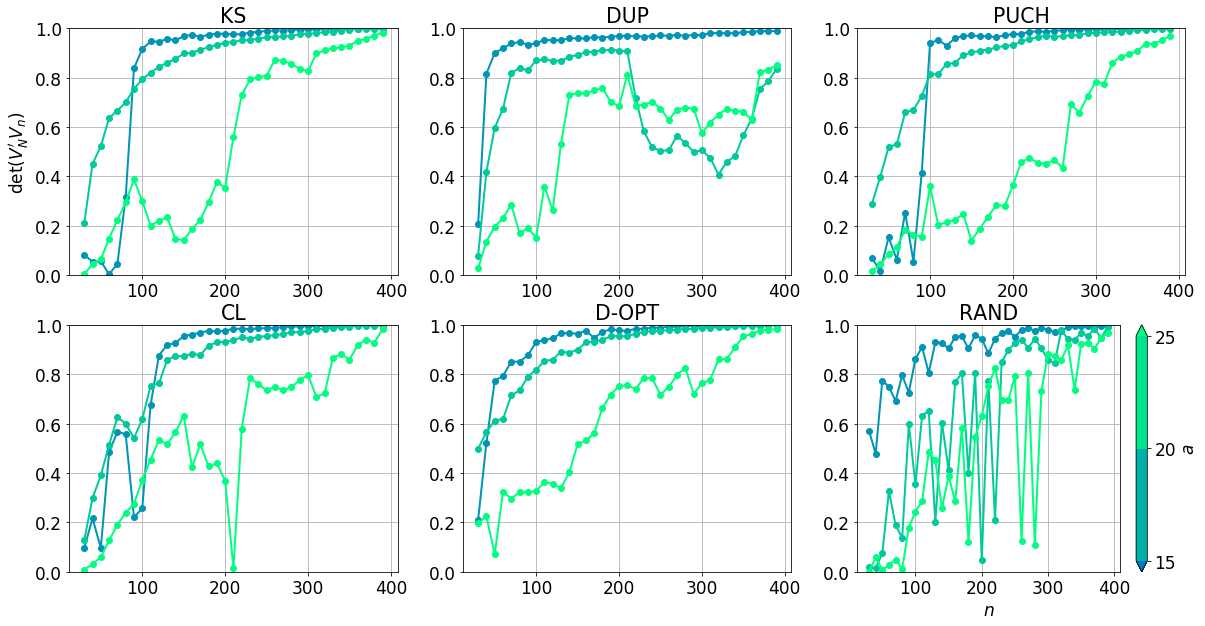
\includegraphics[width=0.6\textwidth]{manuscript/figures/d02_manure_specific_framework_detereigevect.png}}
    \caption{Comparison of eigenvectors when selecting samples with every method and input dimensionality $a=15,20,25$.}
    \label{fig_specific_framework_detereigevect}
\end{figure*}

\begin{figure}[b]
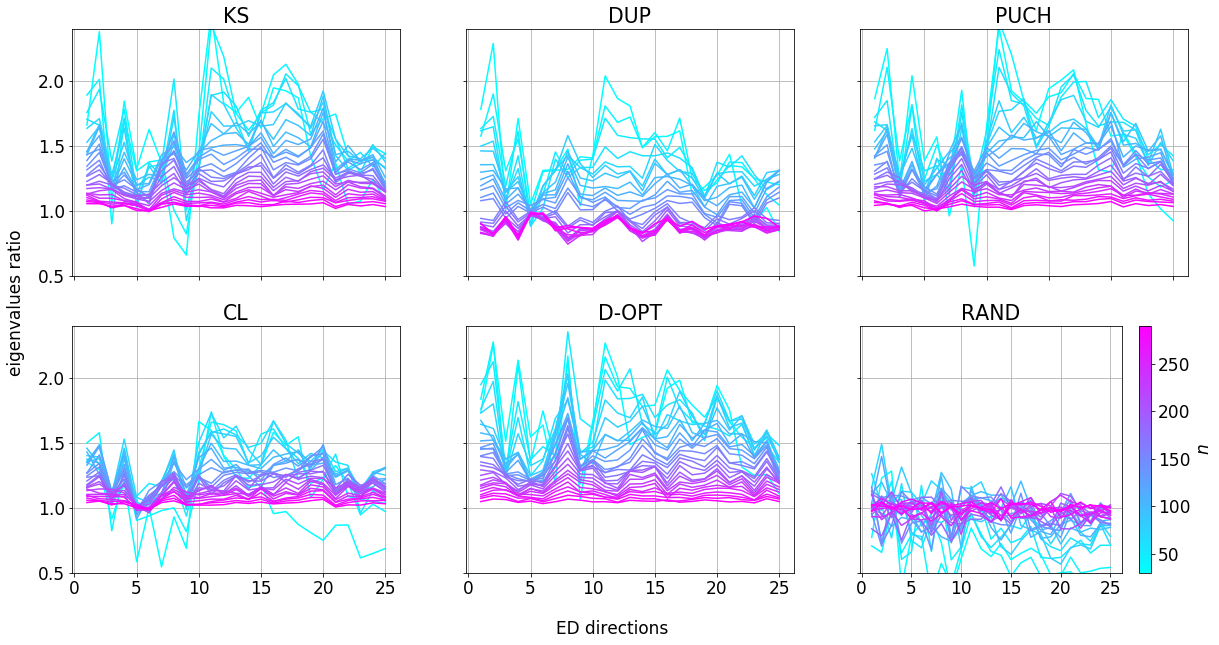
\includegraphics[width=0.8\textwidth]{manuscript/figures/d01_milk_specific_framework_eigenvalsratio.png}
\centering
\caption{Comparison of eigenvalues for Milk when selecting samples with every method and input dimensionality $a=25$.}
\label{fig_d01_milk_specific_framework_eigenvalsratio}
\end{figure}

\begin{figure}[b]
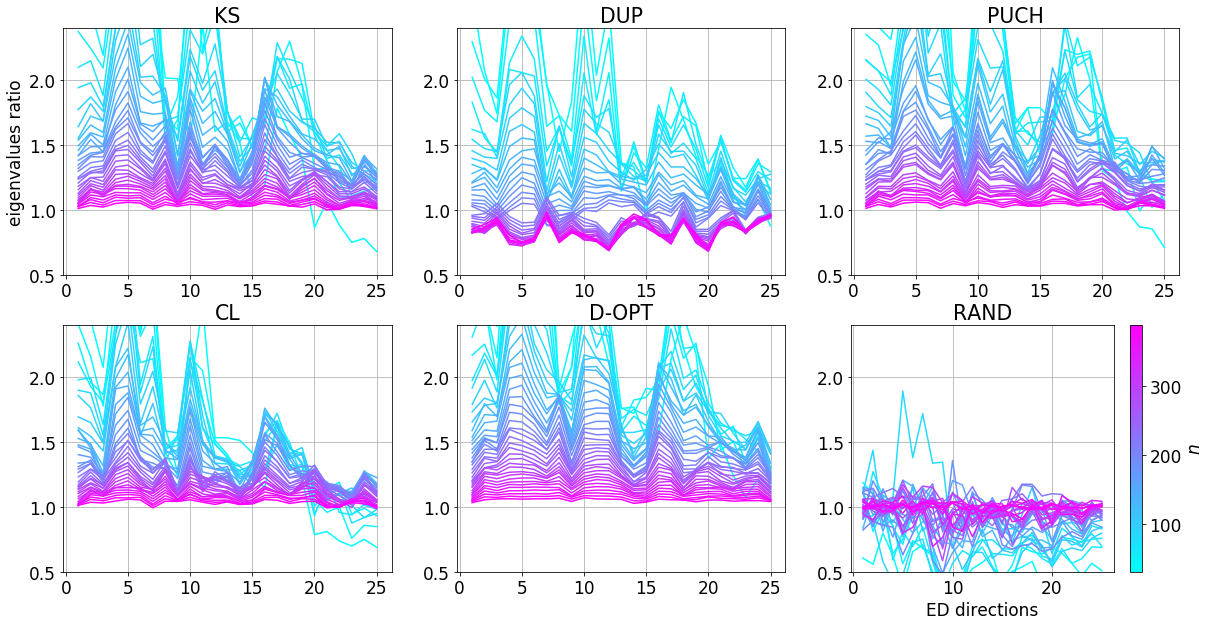
\includegraphics[width=0.8\textwidth]{manuscript/figures/d02_manure_specific_framework_eigenvalsratio.png}
\centering
\caption{Comparison of eigenvalues for Manure when selecting samples with every method and input dimensionality $a=25$.}
\label{fig_d02_manure_specific_framework_eigenvalsratio}
\end{figure}

\subsection*{Model performance}\label{results:modperformance}


\emph{What are the most suitable sample selection conditions in light of satisfactory PLSR models?}

At the aim of connecting the results of the general and the specific framework with the performance of the PLSR calibration models, the RMSEP curves are analyzed in terms of the three factors taken into account: Selection method, input dimensionality and sample size. The motivation to analyze the RMSEP curves is to establish conditions for which the performance of the model stays as close as possible to the result that would be achieved if the PLSR model was built with the complete set of samples. 

The grid in Figures \ref{fig_d01_milk_model_performance} and \ref{fig_d02_manure_model_performance} shows the PLSR model performance for the three factors. The selection methods are accommodated row-wise, punctual sample sizes are positioned column-wise and the color of the curves stands for the input dimensionality as shown in the colorbar. The main insight when comparing both case studies in terms of the impact of the sample selection factors is that the stabilization or convergence of model performance occurs as a function of the number of latent variables. 


\begin{figure}[b]
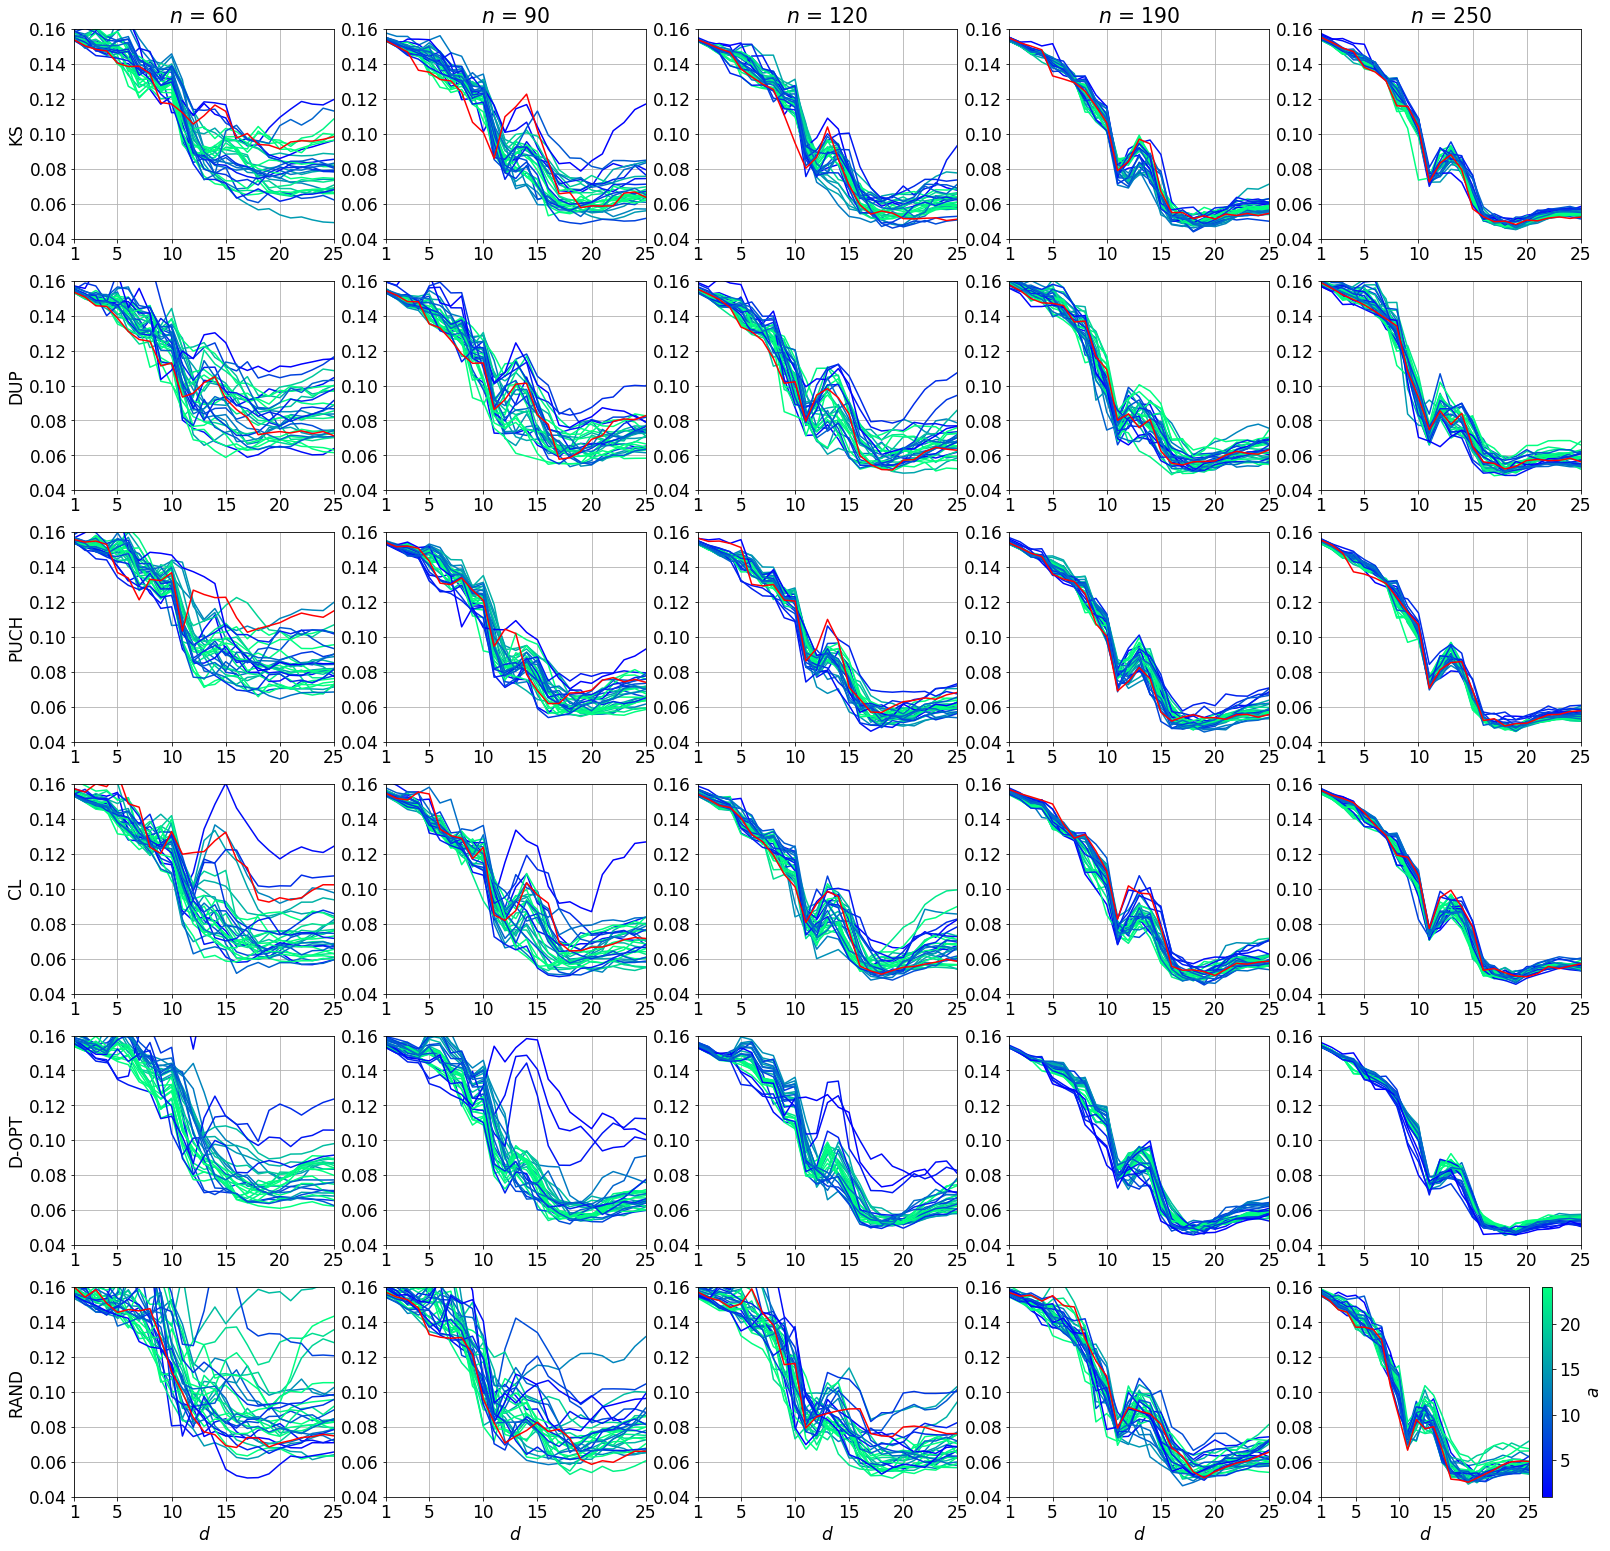
\includegraphics[width=0.8\textwidth]{manuscript/figures/d01_milk_model_performance.png}
\centering
\caption{Model performance to predict lactose according to selection method, input dimensionality and sample size. The red line represents input dimensionality $a=p$.}
\label{fig_d01_milk_model_performance}
\end{figure}

In both cases, RAND selection is clearly more uncertain as the sample size decreases. For higher sample sizes according to the thresholds found in the general framework, RAND selection renders calibration sets that are equally optimal as the sets rendered by any other selection method. In the prediction of lactose, the results for the selected sets of size $n=60$ showed a high variability and no clear relation is found between a satisfactory performance and the selection method or the input dimensionality. Nonetheless, for such a small $n$, the selected set by D-OPT with a large number of $a$ dimensions produced consistently models with better performance. The same result was detected for D-OPT for other small sample sizes ($n=90$ and $n=120$). This differentiation of the effect of the input dimensionality was not equally clear for small sample sizes with the other methods. Moreover, when selecting samples based on the original $\mathbf{X}$ matrix, there was no satisfactory result for the small sample sizes compared to a reduced yet high input dimensionality. When surpassing the threshold and selecting more than 160 samples, the performance of the models with the different methods and input dimensionality stabilized and no important or systematic difference was observed.

The model performance results for the Manure case suggested similar conclusions on the effect of the factors as in the Milk case study. In particular, for a small sample size as $n=60$ D-OPT selection showed a more stable performance  around the optimal number of latent variables with a higher number of SVD dimensions than the other methods. This stabilization by D-OPT was observed more clearly for $n=90$ from 8 to 16 latent variables. The other methods also show stabilization around the same complexities except for RAND and DUP. RAND selection also proved here to render similar results as other selection methods as the sample size increased.




\begin{figure}[b]
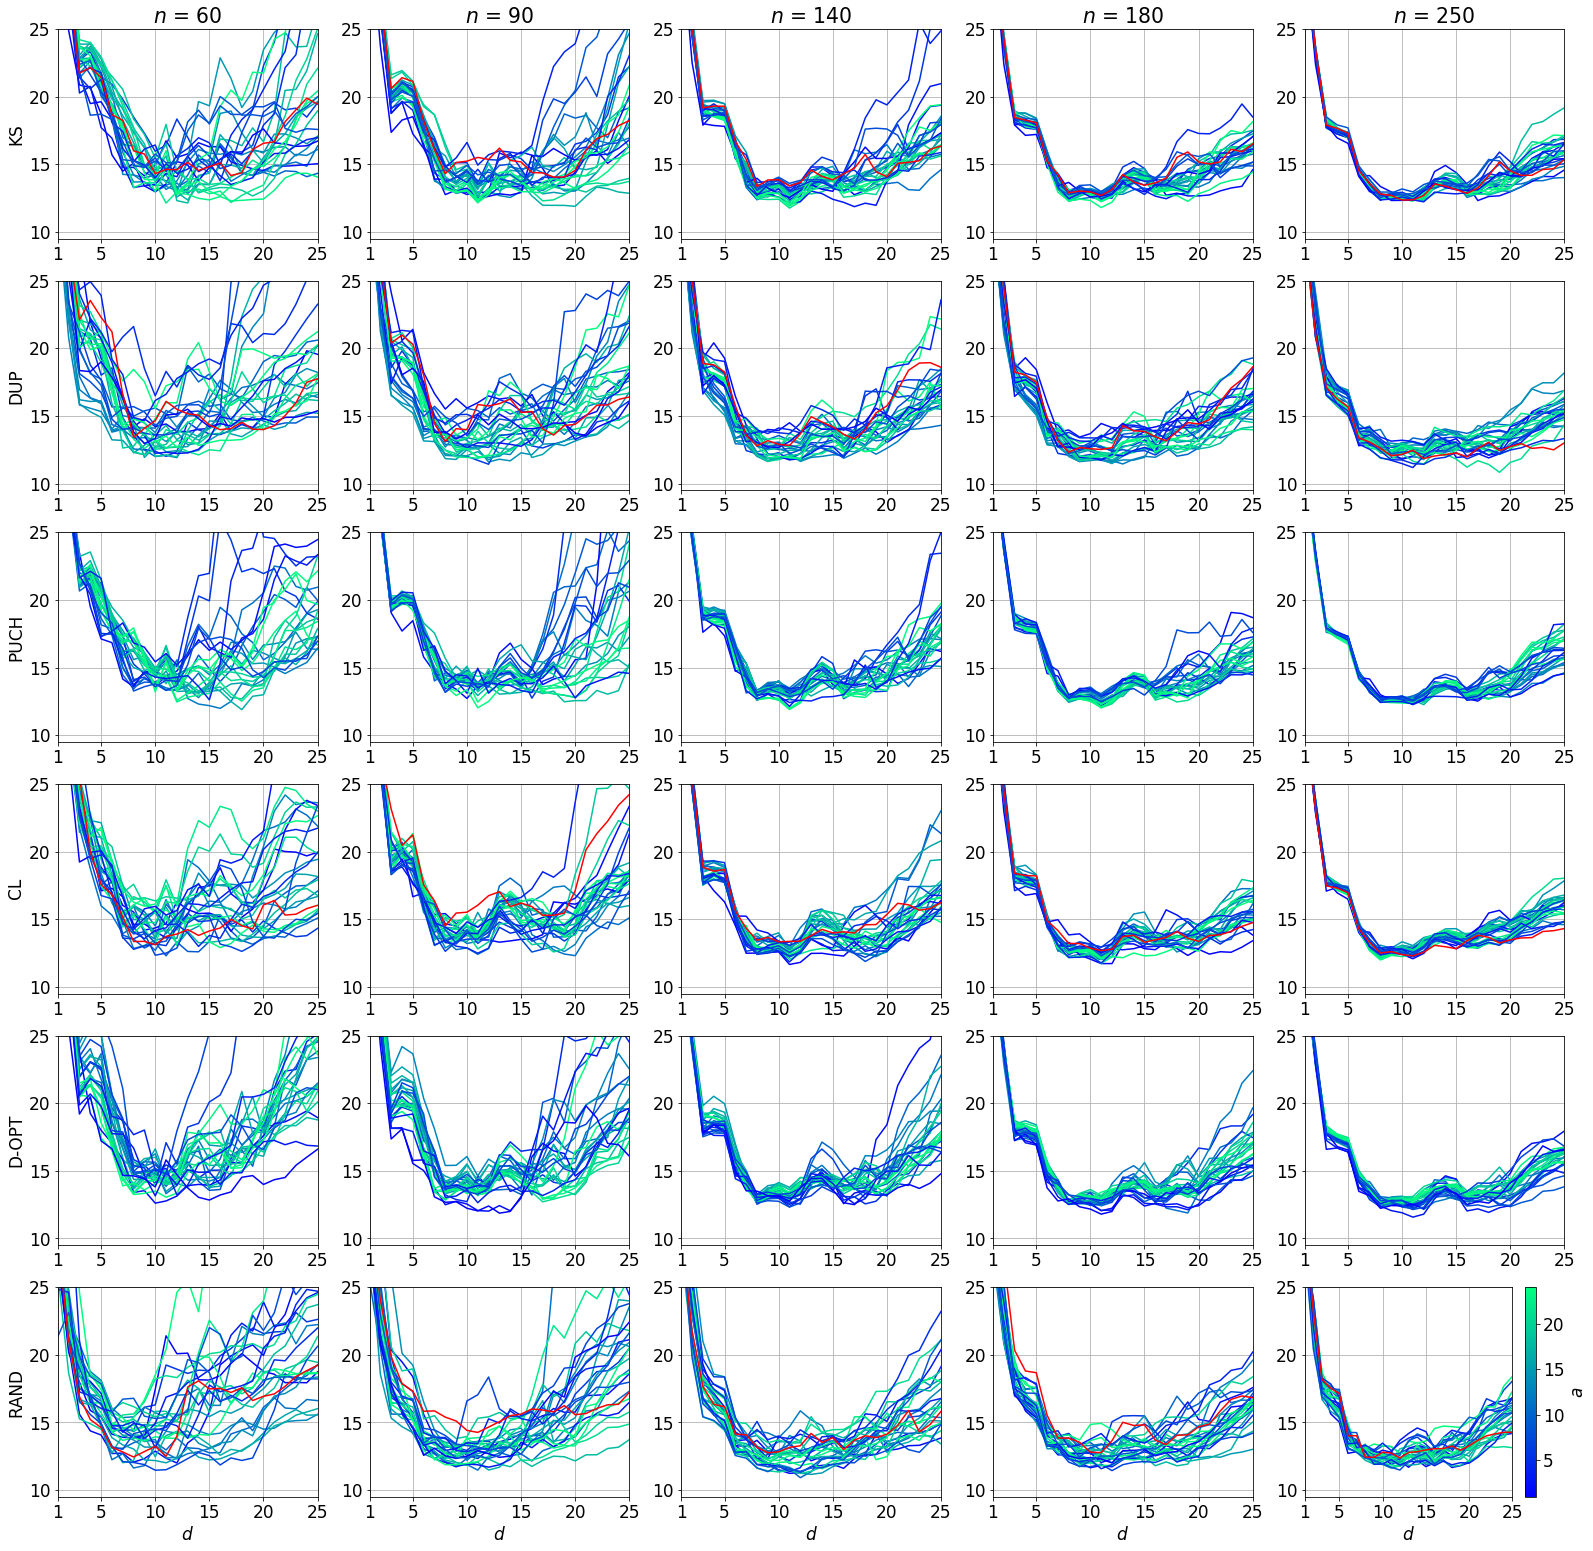
\includegraphics[width=0.8\textwidth]{manuscript/figures/d02_manure_model_performance.png}
\centering
\caption{Model performance to predict DM according to selection method, input dimensionality and sample size. The red line represents input dimensionality $a=p$.}
\label{fig_d02_manure_model_performance}
\end{figure}

% -----------------------------------------------------
% ------------------- discussion  ------------
% -----------------------------------------------------



\section*{Discussion}\label{discussion}

The problem of unsupervised sample selection, although it has been discussed in many previous academic publications, it has not been concretely solved for chemometrics and the type of bilinear models for regression and classification as it was, for example, for linear models in the context of Experimental Design \cite{Brandmaier2012, Goos2011}. The main feature that is always stated to take into account for this problem is that of spanning as much as possible the variability of the samples. Based on the model performance results when selecting samples with a low input dimensionality, it was detected that keeping dimensions of low variability out of sample selection strategy may greatly compromise the performance of the model after gathering reference analyses. This observation was supported by the Pearson correlation values as in the Milk case study, where late PC's presented a high correlation with lactose. In the works that are found in the literature of chemometrics applications, the unsupervised sample selection has been applied with different methods and a reduced input dimensionality, but no analysis is found on the effect of the latter factor \cite{Naes1990, Brandmaier2012, Nawar2018, Au2020}. 

The most claimed feature for sample selection has been that of ``spanning the variability", which until now has not received a clear definition based on the model architectures that are used in multivariate calibration. In the industry, there is still no clear answer on how to approach this step during building calibration models, particularly in terms of sample sizes and the method to select the samples. Based on the model performance results between calibrating with full sample or a reduced but high input dimensionality, it becomes advisable to based the spanning of variability based on the equivalence between covariance matrices $\mathbf{S}_N$ and $\mathbf{S}_n$. However, so far there is no unique mathematical criterion that could translate the SVD equivalence between two matrices with rank $a$ as the equivalence of eigenvectors and subject to eigenvalues ratios as close as possible to 1 from above. Such a criterion would produce a subset of samples equivalent to the full set without underestimating any variability. In an unsupervised selection, good approaches to estimate the real rank of $\mathbf{S}$ are the changes in determinant as seen in Figure \ref{fig_specific_framework_detereigevect} and the predictive power of principal components as discussed in Artemiou (2013) \cite{Artemiou2013}. 

When positioning the PLSR algorithm in the general framework of statistical learning theory, it was found that indeed, the sample size to be considered for multivariate calibration models cannot be thought outside of the $VC$ dimension (i.e. complexity) of the PLSR model. This means that an optimal sample size is not the same for an easy-to-predict chemical constituent as it is for another one that is harder to predict. This was revealed by the optimal sample sizes obtained in each of the case studies. The level of easiness to predict is what the $VC$ dimension or model complexity represents. It was found that indeed, a ratio $n/d>20$ accounts for a sample size that is rather large for a satisfactory calibration model. Based on the results of the present study, for which a hard-to-predict component (lactose) and an easier component (dry matter) were analyzed, we have evidence that a satisfactory calibration model can be found for $n/d>12$. Although in practice the problem of unsupervised sample selection is encountered when there is no data available for the target variable $y$, we believe it is possible to make an estimation based on the literature and expertise of the researchers in charge.

In Au (2020)\cite{Au2020}, there were thresholds found for the optimal sample size in a multivariate calibration application. However, as the sample size steps taken were large, the detected thresholds corresponded to sample sizes for which the ratio $n/d>20$, as the optimal model complexity shown there was about 7 to 10 latent variables. Those results still confirm the theory based on the $n/d$ given by Vapnik \cite{Vapnik2000}.

The specific framework analysis aimed to depict the role that the matrix $\mathbf{S}$ plays when selecting the samples. If the linear relationship holds as modelled and trained by the PLSR algorithm, obtaining $\mathbf{S}_n$ equivalent to $\mathbf{S}_N$ should provide an equivalent calibration model. This may not be the case if strong nonlinearities exist with respect to the chemical component, for which the sample selection problem should be thought with respect to a nonlinear model architecture. The criterion provided by the D-OPT algorithm is indeed the closest to what is needed for matrix equivalence between $\mathbf{S}_n$ and $\mathbf{S}_N$. Yet it is not exactly the same. D-OPT is not design to achieve this.

When connecting this specific framework analysis with the performance of the calibration models it is conclusive that aiming for a larger number of SVD dimensions is more advantageous than restricting it when no information of the $y$ variable is available. In particular, for more difficult components to predict, as it is the case of lactose, it was verified that there is a higher correlation with SVD dimensions of smaller variability than those of highest variability. This of course changes when preprocessing and filters for the signals are applied. But in an unsupervised setting, when the complete variability is available in raw signals, late SVD dimensions play an important role. Therefore, it is advisable to consider a high number of components than restricting it with state-of-the-art selection criteria. In general, it is found that 20 to 30 SVD components contain already certain amount of noise, for which we ensure that no important variability sources for the signals is discarded. In addition to this, it was not found that selecting the samples based on the high dimensionality of the original $\mathbf{X}$ matrix was particularly advantageous than based on the SVD dimensions. This is particularly relevant because D-OPT does not support the original matrix $\mathbf{X}$ when its rank is deficient.

Another feature that is of question when using D-OPT selection is the so-called \emph{effects} to include, concretely, the degree of these effects \cite{Goos2011}. When including only the main effects, D-OPT unavoidably selects the outer layer of the data dispersion in the space. For particular purposes of the theory and applications of Experimental Design, interactions and higher order effects are commonly considered for the sample selection \cite{Brandmaier2012}. However, in multivariate calibration and unsupervised sample selection, we do not have any prior information to motivate the inclusion of other types of effects based on the model architecture of the PLSR model. As it mathematically holds true, the covariance director vector $\mathbf{s}_{xy} = \mathbf{X}'y$ belongs to the space of the covariance matrix $\mathbf{S}$ which also supports the focus on evaluating the equivalence between $\mathbf{S}_n$ and $\mathbf{S}_N$. 

The results on the model performance indicate that if efforts are to be put on the method for selection and input dimensionality, they are relevant for small sample sizes. For large sample sizes, RAND selection did not prove to be different than the subsets selected with other methods.

In terms of preprocessing, several authors still consider specific preprocessing techniques to filter out certain spectral attributes from the signals. For sample selection, previous work was found commenting on the possible advantages of preprocessing the spectral data for unsupervised sample selection \cite{Liu2019}. However, initial experiments in the current case studies suggested that assuming advanced preprocessing such as scattering correction resulted in subsamples rendering poor performance calibration models. Therefore, we believe that strong assumptions prior to obtaining reference analysis is not advisable in general.



% -----------------------------------------------------
% ------------------- conclusions  ------------
% -----------------------------------------------------

\section*{Conclusions}\label{conclusions}
no conclusions yet

% -----------------------------------------------------
% ------------------- acknowledgements  ------------
% -----------------------------------------------------

\begin{acknowledgement}

Valeria Fonseca Diaz is funded as aspirant to doctoral fellow of
the Research Foundation-Flanders (FWO Brussels, Belgium).
The authors thank Dr. Raffaele Vitale and professor Peter Goos (KU Leuven, Belgium) for their suggestions on the conducted analysis given their expertise in Chemometrics and Experimental Design. 
\end{acknowledgement}

% -----------------------------------------------------
% ------------------- bibliography  ------------
% -----------------------------------------------------



\bibliography{biblio}


\end{document}

